\documentclass{beamer}
%
% Choose how your presentation looks.
%
\usepackage[T1]{fontenc}
\usepackage[utf8]{inputenc}
\usepackage{lmodern}  
\usepackage{tikz}%boxy  
\usetikzlibrary{calc}
\usepackage{amsmath}
\usepackage{bm}
\usepackage{graphicx}
\usepackage{booktabs}
\usepackage{multirow}
%
% For more themes, color themes and font themes, see:
% http://deic.uab.es/~iblanes/beamer_gallery/index_by_theme.html
%
\mode<presentation>
{
  \usetheme{Darmstadt}      % or try Darmstadt, Madrid, Warsaw, ...
  \usecolortheme{default} % or try albatross, beaver, crane, ...
  \usefonttheme{serif}  % or try default, serif, structurebold, ...
  \setbeamertemplate{navigation symbols}{}
  \setbeamertemplate{caption}[numbered]
    \setbeamertemplate{headline}{}
} 
%
%
\title[Week1]{Week 5: Estimators and Estimation
Methods, Nonlinear Regression, Quantile Regression}
\author{Advanced Econometrics 4EK608}
\institute{Vysoká škola ekonomická v Praze}
\date{}

\begin{document}
 
\begin{frame}
  \titlepage
\end{frame}

% Uncomment these lines for an automatically generated outline.
\begin{frame}{Outline}
  \tableofcontents
\end{frame}

%---------------------------------------------
\section{Estimators and estimation methods}
\subsection{Properties of estimators - repetition from BSc courses}
\begin{frame}{Estimators and estimation methods}
Notation:
\begin{itemize}
\item $\theta$ - population parameter
\item $(x_1,x_2,\dots,x_n)$ - random sample of $n$ observation of $x$
\item $\hat{\theta}= \hat{\theta}(x_1,x_2,\dots,x_n) ~$ is an estimator of $\theta$
\end{itemize}
Basic notions: 
\begin{itemize}
\item All estimators posses sampling distribution\\
~~mean: $\mathbf{E}(\hat{\theta})$\\
~~variance: $\mathbf{E}[(\hat{\theta}-\mathbf{E}(\hat{\theta}))^2]$\\
~~etc.
\item Estimators $\times$ estimate 
\item Many estimators exist for a parameter (population mean):
\end{itemize}
%\begin{block}{Example}
\begin{align*}
\hat{\theta}_1 & = \overline{x} = \frac{\sum_{i=1}^nx_i}{n}\\
\hat{\theta}_2 & = \tilde{x} = \frac{1}{2}(x_{max} +x_{min})
\end{align*}
\end{frame}


%---------------------------------------------
\begin{frame}{Estimators and estimation methods}
Small sample properties of estimators \& definitions:
\vspace{0.3cm}
\begin{itemize}
\item \textbf{Unbiasedness}: the mean of sampling distribution equals the parameter being estimated
\vspace{0.3cm}
\item \textbf{Efficiency}: an estimator is efficient if it is unbiased and no other
unbiased estimator has a smaller variance. This is usually difficult to prove, that is why we simplify the concept:
\vspace{0.3cm}
\begin{itemize}
\item Relative efficiency
\vspace{0.3cm}
\item Linear unbiased estimators instead of unbiased estimators (linear estimator is linear function of sample observations)
\end{itemize}
\end{itemize}
\end{frame}
%---------------------------------------------
\begin{frame}{Estimators and estimation methods}
Small sample properties of estimators \& definitions:\\
\vspace{0.5cm}
Best Linear Unbiased Estimator (BLUE) is linear, unbiased and no other linear unbiased estimator has a smaller variance. It is not necessarily the best estimator.
\vspace{0.5cm}
\begin{itemize}
\item Non-linear estimators can be better
\item Biased estimators can have smaller Mean Square Error: sum of variance and the squared bias
\end{itemize}
\end{frame}
%---------------------------------------------
\begin{frame}{Estimators and estimation methods}
Large sample properties of estimators \& definitions:
\vspace{0.3cm}
\begin{itemize}
\item Sampling distribution of an estimator changes with the size of sample. 
\vspace{0.3cm}
\item Asymptotic distribution for any estimator is that distribution to which the sampling distribution tends as the sample becomes larger. Its $1^{st}$ and $2^{nd}$ moments are asymptotic mean and asymptotic variance.
\vspace{0.3cm}
\item When the sampling distribution collapses onto a single value when the sample becomes larger, we call this value probability limit. We say estimator converges in probability to that value
\end{itemize}
\end{frame}
%---------------------------------------------
\begin{frame}{Estimators and estimation methods}
Large sample properties of estimators \& definitions:\\
\medskip
\begin{itemize}
\item Asymptotic unbiasedness 
\bigskip
\item \textbf{Consistency} 
\item Unbiased estimators are not necessarily consistent.
\item If $\hat{\theta}$ is an unbiased estimator of $\theta$ and $\textnormal{plim}(\textit{var}(\hat{\theta}))=0$ \\i.e. [ $\textit{var}(\hat{\theta}) \rightarrow 0 \textnormal{ as } n \rightarrow \infty$], then $\textnormal{plim}(\hat{\theta}) = \theta$. 
\item Consistent estimators: unibased \& their variance shrinks to zero as sample size grows (entire population is used).
\begin{itemize}
\item Minimal requirement for estimator used in statistics or econometrics.
\item If some estimator is not consistent, then it does not provide estimates of population $\theta$ values, even with unlimited data.
\end{itemize}
\end{itemize}
\end{frame}
%---------------------------------------------
\begin{frame}{Estimators and estimation methods}
Large sample properties of estimators \& definitions:
\bigskip
\begin{itemize}
\item Asymptotic efficiency: An estimator is asymptotically efficient if it is asymptotically unbiased and no other asymptotically unbiased estimator has smaller asymptotic variance.
\medskip
\item Asymptotic efficiency is usually difficult to prove, that is why we simplify the concept: 
\begin{itemize}
\medskip
\item Relative asymptotic efficiency
\smallskip
\item Linear asymptotically unbiased estimators instead of asymptotically unbiased estimators
\end{itemize}
\end{itemize}
\end{frame}
%---------------------------------------------
\subsection{Method of moments}
\begin{frame}{Estimators and estimation methods}
\textbf{Method of moments}
\medskip
\begin{itemize}
\item With the method of moments, we simply estimate population moments by corresponding sample moments. 
\item Under very general conditions, sample moments are consistent estimators of the corresponding population moments, but NOT necessarily unbiased estimators.
\end{itemize}
\begin{block}{Application example 1}
Sample covariance is a consistent estimator of population covariance.
\end{block}
\begin{block}{Application example 2}
OLS estimators we have used for parameters in the CLRM can be derived by the method of moments. 
\end{block}
\end{frame}
%---------------------------------------------
\begin{frame}{Estimators and estimation methods}
\textbf{Method of moments (MM)}\\
\smallskip
\underline{Population moments}, stochastic variable $X$\\
\begin{itemize}
\item $\mathbf{E}(X^r)$: $r^{th}$ population moment about zero
\item $\mathbf{E}(X)$: the population mean is the first moment about zero
\item $\mathbf{E}[(X-\mathbf{E}(X))^2]$: the population variance is the second moment about the mean
\end{itemize}
\underline{Sample moments}, sample observations $(x_1, x_2, \dots,x_n)$
\begin{itemize}
\item $\frac{\sum_{i=1}^n x^r_i}{n}$: $r^{th}$ sample moment about zero
\item $\frac{\sum_{i=1}^n x_i}{n}=\overline{x} $ : sample mean is the first moment about zero
\item $\frac{\sum_{i=1}^n (x_i-\overline{x})^2}{n-1}$: sample variance is the second sample moment about the mean
\end{itemize}
\end{frame}
%---------------------------------------------
\begin{frame}{Estimators and estimation methods}
\begin{itemize}
\item In a LRM: $\, \hat{y} = \hat{\beta}_0 + \hat{\beta}_1 x_{1} + \dots + \hat{\beta}_k x_{k} \,$, the $k+1$ parameters are \textbf{OLS}-estimated by minimizing:
\footnotesize{
\begin{equation} \label{OLS1}
\sum_{i=1}^n \left( y_i - \hat{\beta}_0 - \hat{\beta}_1 x_{i1} - \dots - \hat{\beta}_k x_{ik} \right)^2
\end{equation}
} %end footnotesize
\item In MM, population moment assumptions $E(u)=0$ and $E(x_j \cdot u)=0$ are used for sample-based estimation (identical to $1^{st}$ order conditions for \eqref{OLS1} - OLS is a type of MM estimator):
\footnotesize{
\begin{equation*}
\begin{aligned}
\sum_{i=1}^n ~~~~\left( y_i - \hat{\beta}_0 - \hat{\beta}_1 x_{i1} - \dots - \hat{\beta}_k x_{ik} \right) &= 0\\
\sum_{i=1}^n  x_{i1} \left( y_i - \hat{\beta}_0 - \hat{\beta}_1 x_{i1} - \dots - \hat{\beta}_k x_{ik} \right) &= 0\\
\dots &\\
\sum_{i=1}^n x_{ik} \left( y_i - \hat{\beta}_0 - \hat{\beta}_1 x_{i1} - \dots - \hat{\beta}_k x_{ik} \right) &= 0\\
\end{aligned}
\end{equation*}
} %end footnotesize
\end{itemize}
\end{frame}
%---------------------------------------------
\begin{frame}{Estimators and estimation methods}
\begin{itemize}
    \item Let $h (\bm{w}) = h(y,\bm{x}, \bm{z}, \bm{\theta})$ define a regression model,
    \\so that $ E h [( y_i, \bm{x}_i, \bm{z}_i, \bm{\theta} )] = 0 \, , ~~~ \forall i.$ 
    \\where $\bm{z}$ is a set of $r$ instruments (IVs) - see Week 8.
    \\For simplicity, we can start by assuming  $\bm{x} \equiv \bm{z}$.
    \item \textbf{Method of moments estimator} $\hat{\bm{\theta}}_{\textit{MM}}$ minimizes:
    $$
    \underset{\hat{\bm{\theta}}}{\textnormal{min}}:
    \left[ \frac{1}{n} \sum_{i=1}^n h (\bm{w}_i,\hat{\bm{\theta}} )
    \right]^{\prime}
    \left[ \frac{1}{n} \sum_{i=1}^n h (\bm{w}_i,\hat{\bm{\theta}} )
    \right]
    $$
    \item If $\bm{x} \neq \bm{z}$ and \# IVs > \# regressors (overidentification), \textbf{Generalized method of moments} is used (GMM)
    $$
    \underset{\hat{\bm{\theta}}}{\textnormal{min}}:
    \left[ \frac{1}{n} \sum_{i=1}^n h (\bm{w}_i,\hat{\bm{\theta}} )
    \right]^{\prime} \bm{W}_n
    \left[ \frac{1}{n} \sum_{i=1}^n h (\bm{w}_i,\hat{\bm{\theta}} )
    \right]
    $$
    where $\bm{W}_n$ is a conveniently chosen ($r \times r$) matrix. 
    \\ \small{(any positive definite matrix that may depend on data but not on $\theta$, e.g. $I_r$. Optimum $\bm{W}_n$: see e.g. Greene, chapter. 13.4.2)}
\end{itemize}
\end{frame}
%---------------------------------------------
\begin{frame}{Estimators and estimation methods}
\textbf{MM - consistency conditions}\\
\medskip
\begin{itemize}
  \item \textbf{Convergence of the moments:} Sample moments converge in probability to their population counterparts.
  \medskip
  \item \textbf{Identification:} Parameters are identified in terms of the moment equations.
  \begin{itemize}
      \item \textbf{Order condition:} \# IVs $\geq$ \# model variables.
      \item \textbf{Rank condition:} Moment equations are not redundant
      \item Identification will be discussed in detail during Week 8
  \end{itemize}
  \medskip
  \item \textbf{Limiting Normal distribution for the sample moments:} Population moments obey central limit theorem (CLT) or some similar variant.
\end{itemize}
\end{frame}
%---------------------------------------------
\begin{frame}{Estimators and estimation methods}
\textbf{MM - summary}\\
\begin{itemize}
\item MM is robust to differences in ``specification'' of the data generating process (DGP). $\rightarrow$ i.e. sample mean or sample variance estimate their population counterparts (assuming they exist) regardless of DGP.
\medskip
\item MM is free from distributional assumptions.
\medskip
\item ``Cost'' of this approach: if we know the specific distribution of a DGP, MM does not make use of such information $\rightarrow$ inefficient estimates.
\medskip 
\item Alternative approach: method of maximum likelihood utilizes distributional information and is more efficient (provided this information is valid).
\end{itemize}
\end{frame}
%---------------------------------------------
\subsection{Maximum likelihood estimation}
\begin{frame}{Estimators and Estimation Methods}
\textbf{Maximum likelihood estimator}\\
\medskip
Single $\theta$ parameter case:\\
\begin{itemize}
\item $1^{st}$ step: deriving a likelihood function $L=L(\theta ,y_1, y_2, ... , y_n)$, where $y_i$ is observation of $Y$ (stochastic), $\theta$ is parameter of the distribution.\\
\item $2^{nd}$ step: finding maximum of $L$ with respect to $\theta$, \\that maximum is $\tilde{\theta} = \theta_{MLE}$
\end{itemize}
With more parameters: $\bm{\theta} = (\theta_1, \dots , \theta_m)^{\prime}$
$$L=L(\theta_1, \theta_2, ... \theta_m, y_1, y_2, ... , y_n)$$
We find MLEs of the $m$ parameters by partially differentiating the likelihood function $L$ with respect to each $\theta$ and then setting all the partial derivatives obtained to zero.\\
\end{frame}
%---------------------------------------------
\begin{frame}{Estimators and estimation methods}
Likelihood function:\\ 
$f(y_1,y_2,\dots,y_n|\bm{\theta}) = \prod_{i=1}^n f(y_i|\bm{\theta}) = L(\bm{\theta}|\bm{y})$ \\
where $f(y|\bm{\theta})$ is the pdf of $y$, conditioned on set of parameters $\bm{\theta}$.\\
\medskip
\centerline{\underline{Maximum likelihood estimation of CLRM parameters:}}
\begin{align*}
\textnormal{CLRM: } y_i= \alpha + \beta x_i + \varepsilon_i \qquad \mathbf{E}(y_i) & =\alpha +\beta x_i = \bm{x}_i^{\prime}\bm{\beta}\\
\textit{var}(y_i) & =\textit{var}(\varepsilon_i)=\sigma^2
\end{align*}
Probability density function for \textbf{Normal distribution}:\\
\medskip
$f(y|\bm{\theta})=(2\pi\sigma^2)^{-0.5} \hspace{0.1cm} exp[-(y-\mu)^2/2\sigma^2]$\\
\bigskip
In the case of CLRM, for each $y_i=\alpha + \beta x_i + \varepsilon_i$: \\
\medskip
$f(y_i| \bm{x}_i,\bm{\theta})=(2\pi\sigma^2)^{-0,5} \hspace{0.1cm} exp[-(y_i-\mathbf{E}(y_i))^2/2\sigma^2]$, that is:\\
$f(y_i| \bm{x}_i,\bm{\theta})=(2\pi\sigma^2)^{-0,5} \hspace{0.1cm} exp[-(y_i-\bm{x}_i^{\prime}\bm{\beta})^2/2\sigma^2]$

\end{frame}
%---------------------------------------------
\begin{frame}{Estimators and estimation methods}
Log-likehood ($LL$) function, \textbf{Normal distribution} assumed,\\
estimation of CLRM parameters:\\
\begin{align*}
log L(\bm{\theta}|\bm{y}, \bm{X} ) & =\sum_{i=1}^n log[f(y_i|\bm{x}_i, \bm{\theta})] = \\
& = -\frac{1}{2} \sum_{i=1}^n \left\lbrace { log(2\pi) + log(\sigma^2)+\frac{1}{\sigma^2}[y_i-\bm{x}_i^{\prime}\bm{\beta}]^2} \right\rbrace = \\ 
& = -\frac{n}{2}log(2\pi)-\frac{n}{2}log(\sigma^2)-\frac{1}{2\sigma^2} \sum_{i=1}^n [y_i-\bm{x}_i^{\prime}\bm{\beta}]^2
\end{align*}
\\ \bigskip
numerical iterative method is used for $\bm{\theta}=(\alpha, \beta, \sigma^2)$ estimation\\
(by maximizing the log-likelihood function).\\
if CLRM assumptions hold $\Rightarrow$ MLE estimators $\tilde{\alpha}$, $\tilde{\beta}$ and $\tilde{\sigma}^2$\\ are identical to OLS-generated estimators $\hat{\alpha}$, $\hat{\beta}$ (and $\hat{\sigma}^2$).
\end{frame}
%---------------------------------------------
\begin{frame}{Estimators and Estimation Methods}
\textbf{Basic MLE assumptions}\\
\begin{itemize}
    \item \textbf{Parameter space:} Gaps and nonconvexities in parameter spaces would generally collide with estimation algorithms (settings such as $\sigma^2 > 0$ are OK).
    \item \textbf{Identifiability:} The parameter vector $\bm{\theta}$ is identified (estimable), if for two vectors, $\bm{\theta}^{*} \neq \bm{\theta}$ and for some data observations $\bm{x}$, $L(\bm{\theta}^{*}|\bm{x}) \neq L(\bm{\theta}|\bm{x})$.
    \item \textbf{Well-behaved data:} Laws of large numbers (LLN) apply. Some form of CLT can be applied to the gradient (i.e. for the estimation method).
    \item \textbf{Regularity conditions:} ``well behaved'' derivatives of $f(y_i|\bm{\theta})$ with respect to $\bm{\theta}$ (see Greene, chapter 14.4.1).
\end{itemize}
\end{frame}
%---------------------------------------------
\begin{frame}{Estimators and Estimation Methods}
\textbf{MLE properties}\\
\begin{itemize}
    \item \textbf{Consistency:} $\textnormal{plim}(\hat{\bm{\theta}}) = \bm{\theta}_0$ ~~($\bm{\theta}_0$ is the true parameter)
    \medskip
    \item \textbf{Asymptotic normality} of $\bm{\hat{\theta}}$
    \medskip
    \item \textbf{Asymptotic efficiency:}  $\bm{\hat{\theta}}$ is asymptotically efficient and achieves the Cramér-Rao lower bound for consistent estimators (see Greene, chapter 14.4.5)
    \medskip
    \item \textbf{Invariance:} MLE of $\bm{\gamma}_0=\bm{c}(\bm{\theta}_0)$ is $\bm{c}(\bm{\hat{\theta}})$ if $\bm{c}(\bm{\theta}_0)$ \\is a continuous and countinuously differentiable function.
\end{itemize}
\end{frame}
%---------------------------------------------
\begin{frame}{Estimators and estimation methods}
\textbf{MLE - summary}\\
\begin{itemize}
\item MLE is only possible if we know the form of the probability distribution function for the population (Normal, Poisson, Negative Binomial, etc.).
\medskip
\item MLEs possess the large sample properties of consistency and asymptotic efficiency. There is no guarantee that they possess any desirable small-sample properties. 
\medskip
\item Under CLRM assumptions, MLE estimator are identical to OLS estimators.
\medskip
\item MLE-related tests (Likelihood ratio, Wald, LM) will be discussed separately, with reference to a specific model type (e.g. LDVs in Weeks 11 to 13).
\end{itemize}
\end{frame}
%---------------------------------------------
\section{Nonlinear regression models}
\begin{frame}{Nonlinear regression: linear vs. nonlinear models}
\textbf{Linear model:}
$$
y_i = \bm{x}_i^{\prime}\bm{\beta} + \varepsilon_i
$$
\textbf{Nonlinear model:}
$$
~~~~~y_i = h(\bm{x}_i\, , \,\bm{\beta}) + \varepsilon_i
$$
\begin{itemize}
    \item Linear model is a special case of the nonlinear model.
    \item Linear models are linear in parameters \\(encompass regressors such as $x_i^2$, etc.)
    \item Many nonlinear model may be transformed into linear models (log-transformation)
    \item For nonlinear models, nonlinear LS (NLS) are available.
    \item $\partial h(\bm{x}_i\, , \,\bm{\beta})/\partial \bm{x}$ is no longer equal to $\bm\beta$ \\
    (interpretation based on estimated model \dots)
\end{itemize}
\end{frame}
%---------------------------------------------
\begin{frame}{Nonlinear regression}
\textbf{Assumptions of the nonlinear regression model}\\
\begin{itemize}
 \item[1] \textbf{Functional form:} The conditional mean function for $y_i$, given $\bm{x}_i$ is: $$\mathbf{E}[y_i|\bm{x}_i] = h(\bm{x}_i\, , \,\bm{\beta})~, \quad i=1,2,\dots,n$$
 \item[2] \textbf{Identifiability of model parameters:} The parameter vector in the model is identified (estimable) if there is no nonzero parameter $\bm{\beta}^0 \neq \bm{\beta}$ such that $h(\bm{x}_i, \bm{\beta}^0)=h(\bm{x}_i, \bm{\beta})$ for all $\bm{x}_i$.
 \medskip
 \item[3] \textbf{Zero mean of the disturbance:} For $y_i = h(\bm{x}_i\, , \,\bm{\beta}) + \varepsilon_i$, we assume $$
 \mathbf{E}[\varepsilon_i| h(\bm{x}_i\, , \,\bm{\beta})] = 0~, \quad i=1,2,\dots,n
 $$
 i.e. disturbance at observation $i$ is uncorrelated with the conditional mean function.
\end{itemize}
\end{frame}
%---------------------------------------------
\begin{frame}{Nonlinear regression}
\textbf{Assumptions of the nonlinear regression model}\\
\medskip
\begin{itemize}
 \item[4] \textbf{Homoskedasticity and nonautocorrelation:}\\
 \medskip
 conditional homoskedasticity:
 $$
 \mathbf{E}[\varepsilon_i^2| h(\bm{x}_i\, , \,\bm{\beta})] = \sigma^2, \quad i=1,2,\dots,n
 $$
 nonautocorrelation:
 $$
 \mathbf{E}[\varepsilon_i\varepsilon_j| h(\bm{x}_i\, , \,\bm{\beta}), h(\bm{x}_j\, , \,\bm{\beta})] = 0, \quad \textnormal{for all~}i\neq j
 $$
\end{itemize}
\end{frame}
%---------------------------------------------
\begin{frame}{Nonlinear regression}
\textbf{Assumptions of the nonlinear regression model}\\
\medskip
\begin{itemize}
\item[5] \textbf{Data generating process:} DGP for $\bm{x}_i$ is assumed to be a well-behaved population such that first and second sample moments of the data can be assumed to converge to fixed, finite population counterparts. The crucial assumption is that the process generating $\bm{x}_i$ is strictly exogenous to that generating $\varepsilon_i$
\item[6] \textbf{Underlying probability model} There is a well-defined probability distribution generating $\varepsilon_i$. At this point, we assume only that this process produces a sample of uncorrelated, identically (marginally) distributed random variables $\varepsilon_i$ with mean zero and variance $\sigma^2$ conditioned on $h(\bm{x}_i, \bm{\beta})$. Thus, at this point, our statement of the model is \textbf{semi-parametric}.
\end{itemize}
\end{frame}
%---------------------------------------------
\begin{frame}{Nonlinear Regression: NLS}
\textbf{NLS: estimator of the nonlinear regression model}\\
\bigskip
\begin{itemize}
\item NLS: \qquad min:~~ $S(\bm{\beta})=\sum[y_i-h(\bm{x}_i, \bm{\beta})]^2$
\medskip
\item Using standard procedure, we can get $k$ first order conditions for the minimization:
$$
\frac{\partial S(\bm{\beta})}{\partial \bm{\beta} } = 
\sum_{i=1}^n \, [y_i-h(\bm{x}_i, \bm{\beta})] 
\frac{\partial h(\bm{x}_i\, , \,\bm{\beta})]}{\partial \bm{\beta}}
= \bm{0}
$$

\end{itemize}
\smallskip
\begin{itemize}
\item The above first order conditions are also moment conditions and this defines the NLS estimator as a GMM estimator.
\end{itemize}
\end{frame}
%---------------------------------------------
\begin{frame}{Nonlinear regression: NLS}
\textbf{NLS: estimator of the nonlinear regression model}\\
\bigskip
\begin{itemize}
\item NLS being a GMM estimator allows us to deduce that the NLS estimator has good large sample properties: consistency and asymptotic normality (if assumptions are fulfilled).
\medskip
\item Hypothesis testing: The principal testing procedure is the Wald test, which relies on the consistency and asymptotic normality of the estimator. Likelihood ratio and LM tests can also be constructed.
\end{itemize}
\end{frame}
%---------------------------------------------

\begin{frame}{Nonlinear regression: computing NLS estimates}
For nonlinear models, a closed-form solution (NLS estimator) usually does not exist.\\
\medskip
\begin{itemize}
\item Most of the nonlinear maximization problems are solved by an \textbf{iterative algorithm}.
\item The most commonly used of iterative algorithms are \textbf{gradient methods}.
\item The template for most gradient methods in common use is the \textbf{Newton's method}.
\item Look at your software packages which methods are available for computing NLS estimates.
\end{itemize}
\end{frame}
%---------------------------------------------

\begin{frame}{Nonlinear regression: computing NLS estimates}
Examples 7.4 \& 7.8 (Greene):\\ Analysis of a Nonlinear Consumption Function\\
%OLS \\
NLS with starting values equal to 0 \\NLS with starting values equal to the parameters from the OLS estimation (c(3) equal to 1).
%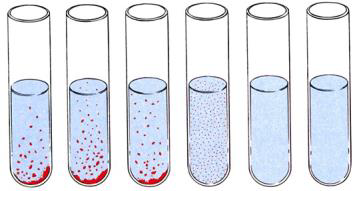
\includegraphics[width=\textwidth, height=6cm]{Obrazek1}
\tiny
\begin{table}[]
\centering
%\caption{My caption}
%\label{my-label}
\begin{tabular}{@{}lllll@{}}
\toprule
\multicolumn{5}{l}{\multirow{6}{*}{\begin{tabular}[c]{@{}l@{}}Depednent Variable: REALCONS\\ Method: Least Squares (Marquard - EViews legacy)\\ Date: 09/19/16 Time 16:31\\ Sample 1950Q1 2000Q4\\ Included observations: 204\\ REALCONS=C(1)+C(2)*REALDPI \\
\midrule
\end{tabular}}} \\
\multicolumn{5}{l}{}                                                                                                                                                                                                                                                       \\
\multicolumn{5}{l}{}                                                                                                                                                                                                                                                       \\
\multicolumn{5}{l}{}                                                                                                                                                                                                                                                       \\
\multicolumn{5}{l}{}                                                                                                                                                                                                                                                       \\
\multicolumn{5}{l}{}                                                                                                                                                                                                                                                       \\ \midrule
                                                           & Coeficient                                         & Std.Error                                         & t-Statistic                                        & Prob.                                           \\
\midrule
C(1)                                                       & -80.35475                                          & 14.30585                                          & -5.616915                                          & 0.0000                                          \\
C(2)                                                       & 0.921686                                           & 0.003872                                          & 238.0540                                           & 0.0000 
\\ \midrule
R-squared                                                  & 0.996448                                           & \multicolumn{2}{l}{Mean dependent var}                                                                 & 2999.436                                        \\
Adjusted R-squared                                         & 0.996431                                           & \multicolumn{2}{l}{S.D. dependent var}                                                                 & 1459.707                                        \\
S.E. of regression                                         & 87.20983                                           & \multicolumn{2}{l}{Akaike info criterion}                                                              & 11.78427                                        \\
Sum squared resid                                          & 1536322                                            & \multicolumn{2}{l}{Schwarz criterion}                                                                  & 11.81680                                        \\
Log likelihood                                             & -1199.995                                          & \multicolumn{2}{l}{Hannan-Quinn criter.}                                                               & 11.79743                                        \\
F-statistics                                               & 56669.72                                           & \multicolumn{2}{l}{Durbin-Watson stat}                                                                 & 0.092048                                        \\
Prob(F-statistics)                                         & 0.000000                                           & \multicolumn{2}{l}{}                                                                                   &                                                 \\ \bottomrule
\end{tabular}
\end{table}
\end{frame}
%---------------------------------------------
\begin{frame}{Nonlinear regression: computing NLS estimates}
Examples 7.4 \& 7.8 (Greene): \\Analysis of a Nonlinear Consumption Function\\
%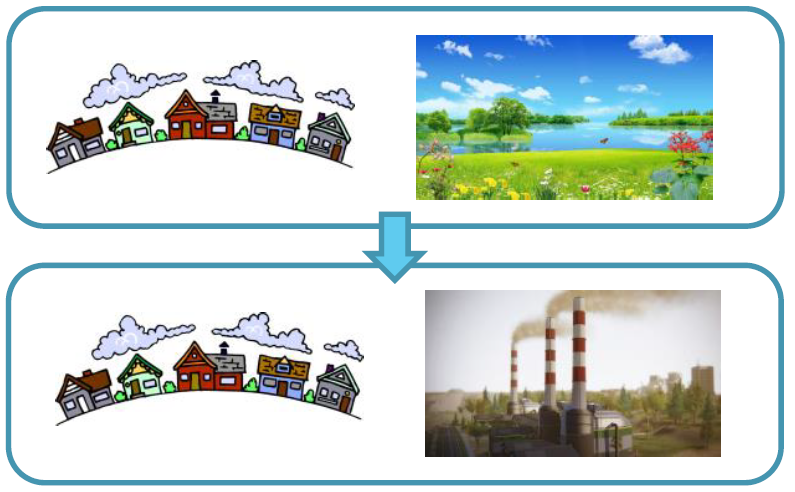
\includegraphics[width=\textwidth, height=7cm]{Obrazek2}
\tiny
\begin{table}[]
\centering
%\caption{My caption}
%\label{my-label}
\begin{tabular}{@{}lllll@{}}
\toprule
\multicolumn{5}{l}{\multirow{4}{*}{\begin{tabular}[c]{@{}l@{}}Depednent Variable: REALCONS\\ Method: Least Squares (Marquard - EViews legacy)\\ Sample 1950Q1 2000Q4 \quad Included observations: 204\\ Convergence achieved after 200 iterations\\ REALCONS=C(1)+C(2)*REALDPI\textasciicircum C(3) \\
\end{tabular}}} \\
\multicolumn{5}{l}{}                                                                                                                                                                                                                                                                            \\
\multicolumn{5}{l}{}                                                                                                                                                                                                                                                                            \\
\multicolumn{5}{l}{}                                                                                                                                                                                                                                                                            \\
\multicolumn{5}{l}{}                                                                                                                                                                                                                                                                            \\
\multicolumn{5}{l}{}                                                                                                                                                                                                                                                                            \\ \midrule
                                                             
                                                             & Coeficient                                           & Std.Error                                                    & t-Statistic                                           & Prob.                                              \\ \midrule
C(1)                                                         & 458.7991                                             & 22.50140                                                     & 20.38980                                              & 0.0000                                             \\
C(2)                                                         & 0.100852                                             & 0.010910                                                     & 9.243667                                              & 0.0000                                             \\
C(3)                                                         & 1.244827                                             & 0.012055                                                     & 103.2632                                              & 0.0000                                             \\ \midrule
R-squared                                                    & 0.998834                                             & Mean dependent var                                           &                                                       & 2999.436                                           \\
Adjusted R-squared                                           & 0.998822                                             & \multicolumn{2}{l}{S.D. dependent var}                                                                               & 1459.707                                           \\
S.E. of regression                                           & 50.09460                                             & \multicolumn{2}{l}{Akaike info criterion}                                                                            & 10.68030                                           \\
Sum squared resid                                            & 504403.2                                             & \multicolumn{2}{l}{Schwarz criterion}                                                                                & 10.72910                                           \\
Log likelihood                                               & -1086.391                                            & \multicolumn{2}{l}{Hannan-Quinn criter.}                                                                             & 10.70004                                           \\
F-statistics                                                 & 86081.29                                             & \multicolumn{2}{l}{Durbin-Watson stat}                                                                               & 0.295995                                           \\
Prob(F-statistics)                                           & 0.000000                                             & \multicolumn{2}{l}{}                                                                                                 &                                                    \\ \bottomrule
\end{tabular}
\end{table}
\end{frame}
%---------------------------------------------
\begin{frame}{Nonlinear regression: computing NLS estimates}
Examples 7.4 \& 7.8 (Greene): \\Analysis of a Nonlinear Consumption Function\\
%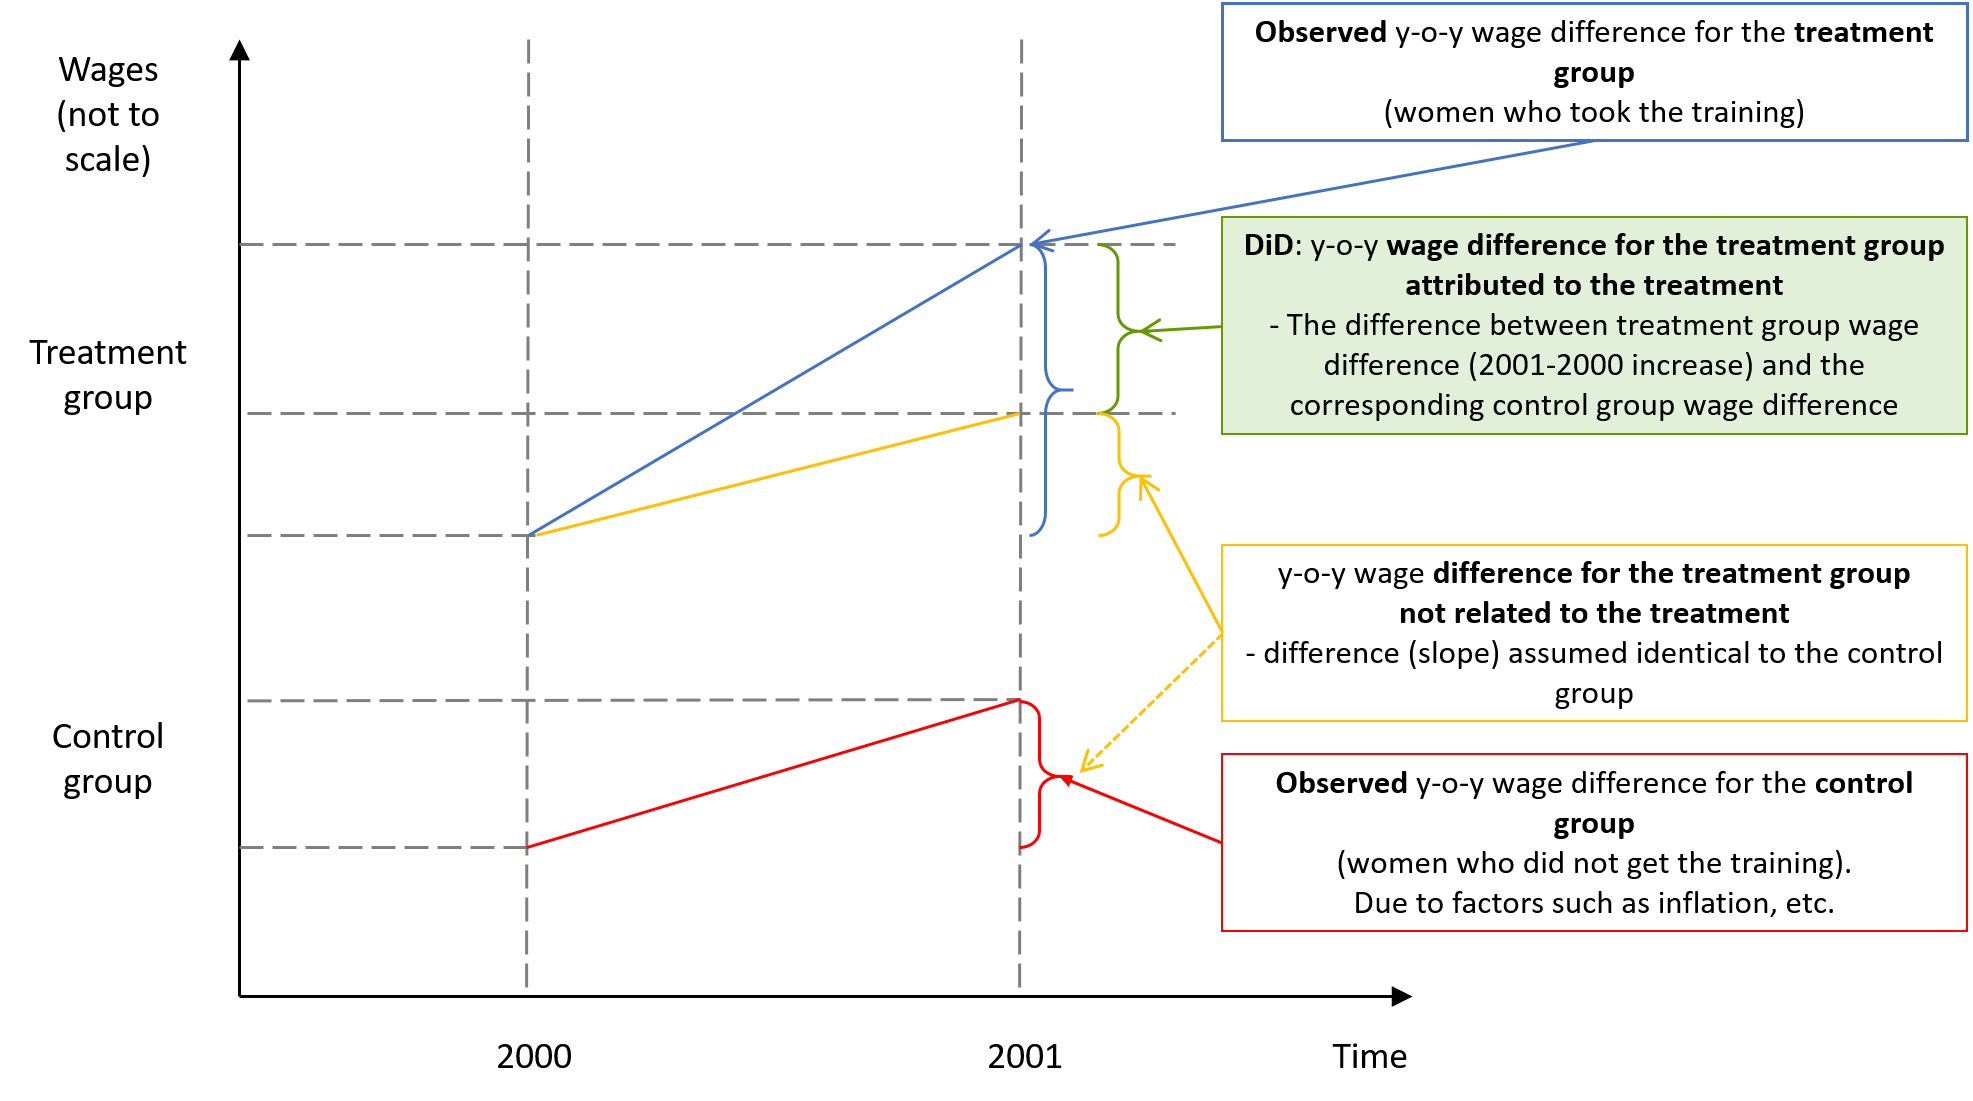
\includegraphics[width=\textwidth, height=7cm]{Obrazek3}
\tiny
\begin{table}[]
\centering
%\caption{My caption}
%\label{my-label}
\begin{tabular}{@{}lllll@{}}
\toprule
\multicolumn{5}{l}{\multirow{4}{*}{\begin{tabular}[c]{@{}l@{}}Depednent Variable: REALCONS\\ Method: Least Squares (Marquard - EViews legacy)\\ Sample 1950Q1 2000Q4 \quad Included observations: 204\\ Convergence achieved after 80 iterations\\ REALCONS=C(1)+C(2)*REALDPI\textasciicircum C(3) \\ \end{tabular}}} \\
\multicolumn{5}{l}{}                                                                                                                                                                                                                                                                                                                       \\
\multicolumn{5}{l}{}                                                                                                                                                                                                                                                                                                                       \\
\multicolumn{5}{l}{}                                                                                                                                                                                                                                                                                                                       \\
\multicolumn{5}{l}{}                                                                                                                                                                                                                                                                                                                       \\
\multicolumn{5}{l}{}                                                                                                                                                                                                                                                                                                                       \\ \midrule
                                                                      & Coeficient                                                    & Std.Error                                                             & t-Statistic                                                   & Prob.                                                      \\ \midrule
C(1)                                                                  & 458.7989                                                      & 22.50149                                                              & 20.38971                                                      & 0.0000                                                     \\
C(2)                                                                  & 0.100852                                                      & 0.010911                                                              & 9.243447                                                      & 0.0000                                                     \\
C(3)                                                                  & 1.244827                                                      & 0.012055                                                              & 103.2632                                                      & 0.0000                                                     \\ \midrule
R-squared                                                             & 0.998834                                                      & Mean dependent var                                                    &                                                               & 2999.436                                                   \\
Adjusted R-squared                                                    & 0.998822                                                      & \multicolumn{2}{l}{S.D. dependent var}                                                                                                & 1459.707                                                   \\
S.E. of regression                                                    & 50.09460                                                      & \multicolumn{2}{l}{Akaike info criterion}                                                                                             & 10.68030                                                   \\
Sum squared resid                                                     & 504403.2                                                      & \multicolumn{2}{l}{Schwarz criterion}                                                                                                 & 10.72910                                                   \\
Log likelihood                                                        & -1086.391                                                     & \multicolumn{2}{l}{Hannan-Quinn criter.}                                                                                              & 10.70004                                                   \\
F-statistics                                                          & 86081.28                                                      & \multicolumn{2}{l}{Durbin-Watson stat}                                                                                                & 0.295995                                                   \\
Prob(F-statistics)                                                    & 0.000000                                                      & \multicolumn{2}{l}{}                                                                                                                  &                                                            \\ \bottomrule
\end{tabular}
\end{table}
\end{frame}
%---------------------------------------------
\section{Quantile regression}
\begin{frame}{Quantile regression (QREG)}
\begin{itemize}
\item Quantile regression estimates the relationship between regressors and a specified quantile of dependent variable.
\medskip
\item The (linear) quantile model can be defined as $Q[y|\bm{x}, q]=\bm{x}^{\prime}\bm{\beta}_q$, such that $\textnormal{Prob}[y \le \bm{x}^{\prime}\bm{\beta}_q|\bm{x}]=q$, $0<q<1$ \\where $q$ denotes the $q$-th quantile.
\medskip
\item One important special case of quantile regression is the least absolute deviations (LAD) estimator, which corresponds to fitting the conditional median of the response variable ($q=\frac{1}{2}$).
\medskip
\item QREG (LAD) estimator can be motivated as a robust  alternative to OLS (with respect to outliers).
\end{itemize}
\end{frame}
%---------------------------------------------
\begin{frame}{Quantile regression (QREG)}
For LRMs, the $q$-th quantile regression estimator $\bm{\beta}_q$ minimizes:
$$
\underset{\bm{\hat{\beta}}_q}{\textnormal{min:}} \quad Q_n(\bm{\hat{\beta}}_q) =
\! \! \sum^n_{i:\, e_i \, \geq \, 0} q|y_i - \bm{x}_i\bm{\hat{\beta}}_q| \,\, +
\! \! \sum^n_{i:\, e_i\, < \, 0} (1-q)|y_i - \bm{x}_i\bm{\hat{\beta}}_q|,
$$
where $e_i = (y_i - \bm{x}_i\bm{\hat{\beta}}_q)$.

\begin{itemize}
    \item We use the notation $\bm{\hat{\beta}}_q$ to make clear that different choices of $q$ lead to different  $\bm{\hat{\beta}}$.
    \item Slope of the loss function $Q_n$ is asymmetrical \\(around $e_i=0$).
    \item The loss function is not differentiable (at $e_i=0$) \\$\rightarrow$ gradient methods are not applicable \\(linear programming can be used).
\end{itemize}
\end{frame}
%---------------------------------------------
\begin{frame}{Quantile regression - LAD}
\begin{itemize}
\item LAD estimator is the QREG for $q=\tfrac{1}{2}$ (median) and the loss function simplifies to: $$
\underset{\bm{\hat{\beta}}_{q}}{\textnormal{min:}} \quad Q_n(\bm{\hat{\beta}}_{q}) =
\sum_{i=1}^n |y_i-\bm{x}_i\bm{\hat{\beta}}_{q}|
$$
\item LAD estimator predates OLS (itself older than 200 years). Until recently, QREG and LAD have seen little use in econometrics, as OLS is vastly easier to compute.
\item Different software packages use a variety of optimization algorithms for QREG/LAD estimation.
\item Linear programming can be used for finding QREG estimates (Koenkerr and Bassett (around 1980).
\end{itemize}
\end{frame}
%---------------------------------------------
\begin{frame}{Quantile regression}

QREG coefficient interpretation example:\\
\bigskip
\begin{itemize}
    \item[(1)] $\textnormal{wage}_i = \beta_0 + u_i$
    \item[(2)] $\textnormal{wage}_i = \beta_0 + \beta_1 \textnormal{female}_i + u_i$
    \item[(3)] $\textnormal{wage}_i = \beta_0 + \beta_1 \textnormal{female}_i + \beta_2 \, \textnormal{exper}_i + u_i$
\end{itemize}
\bigskip
The above equations are estimated by OLS / LAD / QREG:\\
\bigskip
\tiny
\begin{tabular}{|l| l |l |l|}
 \hline
 Coefficient   &     OLS     &   LAD ($q=\tfrac{1}{2}$)   &  QREG ($q=\tfrac{3}{4}$)\\
 \hline 
 (1) $\beta_0$ &   $\hat{\beta}_0=\overline{y}$ & $\hat{\beta}_0=\tilde{\,y\,}$ & $\hat{\beta}_0=Q_3$\\
 & sample mean  & sample median & sample $3^{rd}$ quartile\\
 \hline
 (2) $\beta_0, \beta_0\!+\!\beta_1$ & conditional sample mean & cond. sample median & conditional sample $Q_3$\\
  & wage: male / female & wage: male / female & wage: male / female \\
  \hline
  (3) $\beta_2$ & change in expected mean & change in exp. median & change in expected $Q_3$\\
   & wage for $\Delta\textnormal{exper}=1$ & wage for $\Delta\textnormal{exper}=1$ & wage for $\Delta\textnormal{exper}=1$\\
   \hline
\end{tabular}
\end{frame}
%---------------------------------------------
\begin{frame}{Quantile regression example}
Example 7.9 (Greene): \\Cobb-Douglass Production Function\\
OLS $\rightarrow$ Standardized residuals indicate two outliers $\rightarrow$ LAD
\tiny
\begin{table}[]
\centering
\begin{tabular}{@{}lllll@{}}
\toprule
\multicolumn{5}{l}{\multirow{4}{*}{\begin{tabular}[c]{@{}l@{}}Depednent Variable: LNYN\\ Method: Least Squares\\ Sample 1 25 \\ Included observations: 25\end{tabular}}} \\
\multicolumn{5}{l}{}                                                                                                                                                                                 \\
\multicolumn{5}{l}{}                                                                                                                                                                                 \\
\multicolumn{5}{l}{}                                                                                                                                                                                 \\
\multicolumn{5}{l}{}                                                                                                                                                                                 \\ \midrule
Variable                                     & Coeficient                           & Std.Error                          & t-Statistic                          & Prob.                              \\
\midrule
C                                            & 2.293263                             & 0.107183                           & 21.39582                             & 0.0000                             \\
LNKN                                         & 0.278982                             & 0.080686                           & 3.457639                             & 0.0022                             \\
LNLN                                         & 0.927312                             & 0.012055                           & 9.431359                             & 0.0000                             \\
\midrule
R-squared                                    & 0.959742                             & \multicolumn{2}{l}{Mean dependent var}                                    & 0.771734                           \\
Adjusted R-squared                           & 0.956082                             & \multicolumn{2}{l}{S.D. dependent var}                                    & 0.899306                           \\
S.E. of regression                           & 0.188463                             & \multicolumn{2}{l}{Akaike info criterion}                                 & -0.387663                          \\
Sum squared resid                            & 0.781403                             & \multicolumn{2}{l}{Schwarz criterion}                                     & -0.241398                          \\
Log likelihood                               & 7.845786                             & \multicolumn{2}{l}{Hannan-Quinn criter.}                                  & -0.347095                          \\
F-statistics                                 & 262.2396                             & \multicolumn{2}{l}{Durbin-Watson stat}                                    & 1.937830                           \\
Prob(F-statistics)                           & 0.000000                             & \multicolumn{2}{l}{}                                                      &                                    \\ \bottomrule
\end{tabular}
\end{table}
\end{frame}
%---------------------------------------------
\begin{frame}{Quantile regression example}
Example 7.9 (Greene): Cobb-Douglass Production Function\\
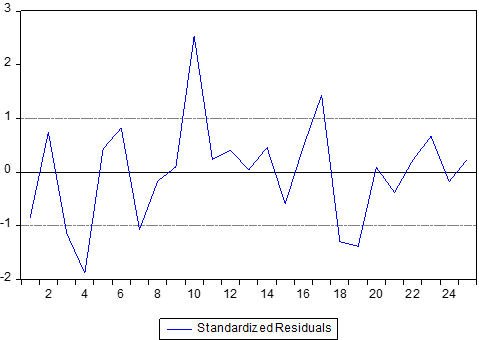
\includegraphics[width=\textwidth, height=7cm]{img/Obrazek5}
\end{frame}
%---------------------------------------------
\begin{frame}{Quantile regression example}
Example 7.9 (Greene): \\Cobb-Douglass Production Function\\
\small{(results differ from the textbook)}
\tiny
\begin{table}[]
\centering
\begin{tabular}{@{}lllll@{}}
\toprule
\multicolumn{5}{l}{\multirow{3}{*}{\begin{tabular}[c]{@{}l@{}}Depednent Variable: LNYN\qquad Method: Quantile Regression (Median)\\  Sample 1 25\qquad Included observations: 25\\ Huber Sandwich Standard Errors \& Covariance\\ Sparsity method: Kemel (Epanechnikov) using residuals\\ Bandwidth method: Hall-Sheather, bw=0.33227\\ Estimation successfully identifies unique optimal solution\end{tabular}}} \\
\multicolumn{5}{l}{}                                                                                                                                                                                                                                                                                                                                                                                                                     \\
\multicolumn{5}{l}{}                                                                                                                                                                                                                                                                                                                                                                                                                     \\
\multicolumn{5}{l}{}                                                                                                                                                                                                                                                                                                                                                                                                                     \\
\multicolumn{5}{l}{}                                                                                                                                                                                                                                                                                                                                                                                                                     \\
\multicolumn{5}{l}{}                                                                                                                                                                                                                                                                                                                                                                                                                     \\ \midrule
Variable                                                                                       & Coeficient                                                                       & Std.Error                                                                       & t-Statistic                                                                       & Prob.                                                                          \\ \midrule
C                                                                                              & 2.275038                                                                         & 0.179268                                                                        & 12.69071                                                                          & 0.0000                                                                         \\
LNKN                                                                                           & 0.260365                                                                         & 0.122447                                                                        & 2.126351                                                                          & 0.0449                                                                         \\
LNLN                                                                                           & 0.927243                                                                         & 0.152593                                                                        & 6.076572                                                                          & 0.0000                                                                         \\ \midrule
Pseudo R-squared                                                                               & 0.794575                                                                         & \multicolumn{2}{l}{Mean dependent var}                                                                                                                              & 0.771734                                                                       \\
Adjusted R-squared                                                                             & 0.775900                                                                         & \multicolumn{2}{l}{S.D. dependent var}                                                                                                                              & 0.899306                                                                       \\
S.E. of regression                                                                             & 0.190505                                                                         & \multicolumn{2}{l}{Objective}                                                                                                                                       & 1.627051                                                                       \\
Quantile dependent va...                                                                       & 0.966677                                                                         & \multicolumn{2}{l}{Restr. objective}                                                                                                                                & 7.920415                                                                       \\
Sparsity                                                                                       & 0.594465                                                                         & \multicolumn{2}{l}{Quasi-LR statistic}                                                                                                                              & 84.69274                                                                       \\
Prob(Quasi-LR stat)                                                                            & 0.000000                                                                         & \multicolumn{2}{l}{}                                                                                                                                                &                                                                                \\ \bottomrule
\end{tabular}
\end{table}
\end{frame}
%---------------------------------------------
\begin{frame}{Quantile regression example 2}
Example 7.10 (Greene): \\Income Elasticity of Credit Cards Expenditure\\
\quad OLS $\quad \& \quad$ LAD $\quad \& \quad$ Income elasticity at different deciles \\
\tiny
\begin{table}[]
\centering
\begin{tabular}{@{}lllll@{}}
\toprule
\multicolumn{5}{l}{\multirow{6}{*}{\begin{tabular}[c]{@{}l@{}}Depednent Variable: LOGSPEND\\ Method: Least Squares\\ Date: 09/15/16 Time 13:53\\ Sample (adjusted): 3 13443\\ Included observations: 10499 after adjustments\end{tabular}}} \\
\multicolumn{5}{l}{}                                                                                                                                                                                                                         \\
\multicolumn{5}{l}{}                                                                                                                                                                                                                         \\
\multicolumn{5}{l}{}                                                                                                                                                                                                                         \\
\multicolumn{5}{l}{}                                                                                                                                                                                                                         \\
\multicolumn{5}{l}{}                                                                                                                                                                                                                         \\ \midrule
Variable                                             & Coeficient                                   & Std.Error                                   & t-Statistic                                  & Prob.                                     \\
\midrule
C                                                    & -3.055807                                    & 0.239699                                    & -12.74852                                    & 0.0000                                    \\
LOGINC                                               & 1.083438                                     & 0.032118                                    & 33.73296                                     & 0.0000                                    \\
AGE                                                  & -0.017364                                    & 0.001348                                    & -12.88069                                    & 0.0000                                    \\
ADEPCNT                                              & -0.044610                                    & 0.010921                                    & -4.084857                                    & 0.0000                                    \\
\midrule
R-squared                                            & 0.100572                                     & \multicolumn{2}{l}{Mean dependent var}                                                     & 4.728778                                  \\
Adjusted R-squared                                   & 0.100315                                     & \multicolumn{2}{l}{S.D. dependent var}                                                     & 1.404820                                  \\
S.E. of regression                                   & 1.332496                                     & \multicolumn{2}{l}{Akaike info criterion}                                                  & 3.412366                                  \\
Sum squared resid                                    & 18634.35                                     & \multicolumn{2}{l}{Schwarz criterion}                                                      & 3.415131                                  \\
Log likelihood                                       & -17909.21                                    & \multicolumn{2}{l}{Hannah-Quinn criter.}                                                   & 3.413300                                  \\
F-statistic                                          & 391.1750                                     & \multicolumn{2}{l}{Durbin-Watson stat}                                                     & 1.888912                                  \\
Prob(F-statistic)                                    & 0.000000                                     & \multicolumn{2}{l}{}                                                                       &                                           \\ \bottomrule
\end{tabular}
\end{table}
\end{frame}
%---------------------------------------------
\begin{frame}{Quantile regression example 2}
Example 7.10 (Greene): \\Income Elasticity of Credit Cards Expenditure (LAD)\\
\tiny
\begin{table}[]
\centering
\begin{tabular}{@{}lllll@{}}
\toprule
\multicolumn{5}{l}{\multirow{6}{*}{\begin{tabular}[c]{@{}l@{}}Depednent Variable: LOGSPEND \quad Method: Quantile Regression (Median)\\  Sample (adjusted): 3 13443\qquad Included observations: 10499 after adjustments\\ Huber Sandwich Standard Errors \& Covariance\\ Sparsity method: Kemel (Epanechnikov) using residuals\\ Bandwidth method: Hall-Sheather, bw=0.04437\\ Estimation successfully identifies unique optimal solution\end{tabular}}} \\
\multicolumn{5}{l}{}                                                                                                                                                                                                                                                                                                                                                                                                                                                          \\
\multicolumn{5}{l}{}                                                                                                                                                                                                                                                                                                                                                                                                                                                          \\
\multicolumn{5}{l}{}                                                                                                                                                                                                                                                                                                                                                                                                                                                          \\
\multicolumn{5}{l}{}                                                                                                                                                                                                                                                                                                                                                                                                                                                          \\
\multicolumn{5}{l}{}                                                                                                                                                                                                                                                                                                                                                                                                                                                          \\ \midrule
Variable                                                                                               & Coeficient                                                                               & Std.Error                                                                              & t-Statistic                                                                              & Prob.                                                                                 \\ \midrule
C                                                                                                      & -2.803756                                                                                & 0.233534                                                                               & -12.00577                                                                                & 0.0000                                                                                \\
LOGINC                                                                                                 & 1.074928                                                                                 & 0.030923                                                                               & 34.76139                                                                                 & 0.0000                                                                                \\
AGE                                                                                                    & -0.016988                                                                                & 0.001530                                                                               & -11.10597                                                                                & 0.0000                                                                                \\
ADEPCNT                                                                                                & -0.049955                                                                                & 0.011055                                                                               & -4.518599                                                                                & 0.0000                                                                                \\ \midrule
Pseudo R-squared                                                                                       & 0.058243                                                                                 & \multicolumn{2}{l}{Mean dependent var}                                                                                                                                            & 4.728778                                                                              \\
Adjusted R-squared                                                                                     & 0.057974                                                                                 & \multicolumn{2}{l}{S.D. dependent var}                                                                                                                                            & 1.404820                                                                              \\
S.E. of regression                                                                                     & 1.346476                                                                                 & \multicolumn{2}{l}{Objective}                                                                                                                                                     & 5096.818                                                                              \\
Quantile dependent va...                                                                               & 4.941583                                                                                 & \multicolumn{2}{l}{Restr. objective}                                                                                                                                              & 5412.032                                                                              \\
Sparsity                                                                                               & 2.659971                                                                                 & \multicolumn{2}{l}{Quasi-LR statistic}                                                                                                                                            & 948.0224                                                                              \\
Prob(Quasi-LR stat)                                                                                    & 0.000000                                                                                 & \multicolumn{2}{l}{}                                                                                                                                                              &                                                                                   \\ \bottomrule
\end{tabular}
\end{table}
\end{frame}
%---------------------------------------------
\begin{frame}{Quantile regression example 2}
Example 7.10 (Greene): \\Income Elasticity of Credit Cards Expenditure\\
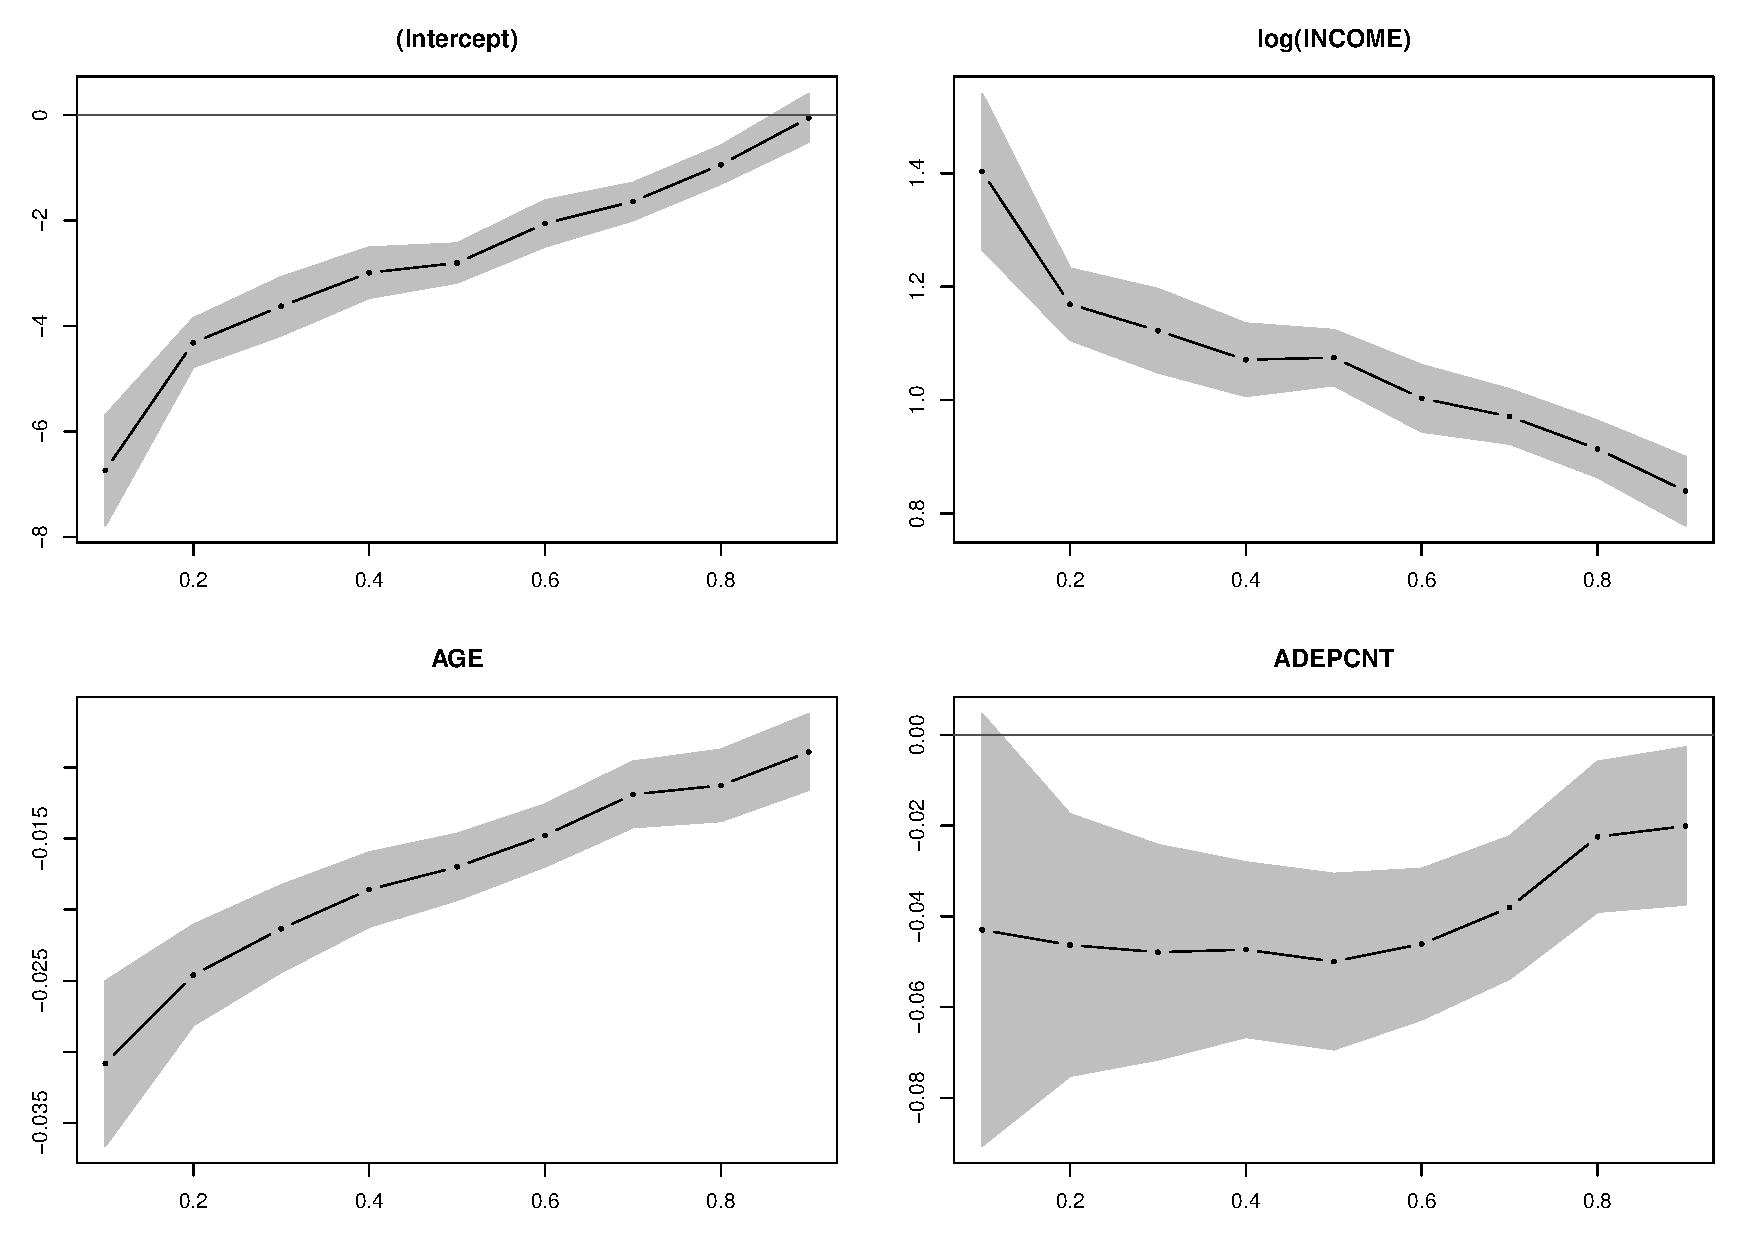
\includegraphics[width=10cm, height=6.7cm]{img/quantil_regression.pdf}
\end{frame}
%---------------------------------
\end{document}